Let us now perform a benchmark simulation of the gradient-based methods.
%
We consider the quantum \acro{tfim}
\begin{equation}
    \label{eq:gradpeps:approx_contraction:results:ising_model}
    H = -\sum_{\langle i, j\rangle} \sigma^x_i \sigma^x_j - g \sum_i \sigma_i^z
\end{equation}
on an $L \times L$ square lattice with open boundary conditions, where $\sigma^\alpha$ denote Pauli operators with eigenvalues $\pm 1$.
%
The model exhibits a phase transition from a $\sigma^x$-ordered ferromagnet for $g < g_c$ to a disordered paramagnet for $g > g_c$ at a critical field strength $g_c \approx 3.05$~\cite{blote2002}.


\subsection{Hamiltonian Representations}
\label{subsec:gradpeps:benchmark:hamiltonian_pepos}
To employ the gradient-based methods, we need to represent the relevant operators in a compatible way, e.g.~as \acrop{pepo}.
%
For ground state search, we can write the Hamiltonian~\eqref{eq:gradpeps:approx_contraction:results:ising_model} either as a sum of $\sim L^2$ bond operators, as a sum of $2L$ \acrop{mpo}, or the sum of $2$ \acrop{pepo}.
%
In the following, we provide explicit constructions for all of these representations.

\paragraph{Sum of bond operators}
First, we find
\begin{equation}
    \label{eq:gradpeps:benchmark:tfim_hamiltonian_as_bond_ops}
    H = \nnsum{i}{j} h^{[ij]}
    \qquad
    h^{[ij]} := - \sigma_i^x \sigma_j^x - \frac{1 + \lambda_{\langle i, j \rangle}}{4}g \sigma_i^z - \frac{1 + \rho{\langle i, j \rangle}}{4}g \sigma_j^z
    ~,
\end{equation}
where $\lambda_{\langle i, j \rangle}, \rho_{\langle i, j \rangle} \in \set{0, 1}$ correct for double counting of sites by setting $\lambda_{\langle i, j \rangle} = 1$ iff site $i$ is at an open boundary and similarly $\rho_{\langle i, j \rangle} = 1$ iff $j$ is at a boundary.


\paragraph{Sum of MPOs}
Alternatively, we may use the finite state machine construction~\cite{crosswhite2008b} to write all terms within a single row or single column as an \acro{mpo}, that is
\begin{align}
\begin{split}
    \label{eq:gradpeps:benchmark:tfim_hamiltonian_as_mpos}
    H = \sum_{x=1}^{L} H^{[x,:]} + \sum_{y=1}^L H^{[:,y]}
    ~,
\end{split}
\end{align}
where the operators act on only a single row (column) and are given as \acrop{mpo} with the following coefficients
\begin{equation}
    \braopket{i_{x,1} \dots i_{x,L}}{H^{[x,:]}}{i'_{x,1} \dots i'_{x,L}}
    ~~ = ~~
    \vcenter{\hbox{\begin{tikzpicture}
        \node[pepo tensor, fill=lime!60] (W1) {};
        \draw (W1.east) -- ++(10pt,0) node[pepo tensor, fill=lime!60, right] (W2) {};
        \draw (W2.east) -- ++(10pt,0) node[pepo tensor, fill=lime!60, right] (W3) {};
        \draw (W3.east) -- ++(10pt,0) node[pepo tensor, fill=lime!60, right] (W4) {};
        \draw (W4.east) -- ++(10pt,0) node[pepo tensor, fill=lime!60, right] (W5) {};
        \draw (W1.west) -- ++(-10pt,0) node[draw, circle, fill=black, inner sep=0, minimum width=.2cm, minimum height=.2cm, left] (vL) {};
        \draw (W5.east) -- ++(10pt,0) node[draw, circle, fill=black, inner sep=0, minimum width=.2cm, minimum height=.2cm, right] (vR) {};
        \node[above=0pt of vL] {$v_L$};
        \node[above=0pt of vR] {$v_R$};
        \draw (W1.north) -- ++(0,5pt) node[above] {$i'_{x,1}$};
        \draw (W2.north) -- ++(0,5pt);
        \draw (W3.north) -- ++(0,5pt);
        \draw (W4.north) -- ++(0,5pt);
        \draw (W5.north) -- ++(0,5pt);
        \draw (W1.south) -- ++(0,-5pt);
        \draw (W2.south) -- ++(0,-5pt);
        \draw (W3.south) -- ++(0,-5pt);
        \draw (W4.south) -- ++(0,-5pt);
        \draw (W5.south) -- ++(0,-5pt) node[below] {$i_{x,L}$};
        \node[above right] at ($(W3.north east) + (0pt,0pt)$) {$C^{[x,y]}$};
    \end{tikzpicture}}}
    .
\end{equation}
The \acro{mpo} tensors are given by
\begin{equation}
    \vcenter{\hbox{\begin{tikzpicture}
        \node[pepo tensor, fill=lime!60] (C) {};
        \node[above left=3pt of C] {$C^{[x,y]}$};
        \draw (C.north) -- ++(0, 5pt);
        \draw (C.south) -- ++(0, -5pt);
        \draw (C.west) -- ++(-10pt,0) node[left] {$\alpha$};
        \draw (C.east) -- ++(10pt, 0) node[right] {$\beta$};
    \end{tikzpicture}}}
    ~~ := ~~
    \begin{pmatrix}
        \eye & \sigma^x & -\tfrac{1}{2}g\sigma^z \\
        0 & 0 & -\sigma^x \\
        0 & 0 & \eye \\
    \end{pmatrix}_{\!\alpha\beta}
    ~,
\end{equation}
where we suppress the physical indices and identify them with the indices that the operator-valued entries of the matrix have in the computational basis.
%
The boundary vectors are $v_L = (1 ~ 0 ~ 0)^\transpT$ and $v_R = (0 ~ 0 ~ 1)^\transpT$.



\paragraph{Sum of PEPOs}
Lastly, we can employ a finite state machine \acro{mpo} construction to form a \acro{pepo} that is the sum of all horizontal \acrop{mpo} above.
%
Note that if we replace a single \acro{mpo} tensor, e.g.~at position $\tilde{y}$ with
\begin{equation}
    \vcenter{\hbox{\begin{tikzpicture}
        \node[pepo tensor, fill=cyan!50] (C) {};
        \node[above left=2pt of C] {$I^{[x,y]}$};
        \draw (C.north) -- ++(0, 5pt);
        \draw (C.south) -- ++(0, -5pt);
        \draw (C.west) -- ++(-10pt,0) node[left] {$\alpha$};
        \draw (C.east) -- ++(10pt, 0) node[right] {$\beta$};
    \end{tikzpicture}}}
    ~~ := ~~
    \begin{pmatrix}
        0 & 0 & \eye \\
        0 & 0 & 0 \\
        0 & 0 & 0 \\
    \end{pmatrix}_{\!\alpha\beta}
    ,
\end{equation}
the modified \acro{mpo}
\begin{equation}
    \vcenter{\hbox{\begin{tikzpicture}
        \node[pepo tensor, fill=lime!60] (W1) {};
        \draw (W1.east) -- ++(10pt,0) node[pepo tensor, fill=lime!60, right] (W2) {};
        \draw (W2.east) -- ++(10pt,0) node[pepo tensor, fill=lime!60, right] (W3) {};
        \draw (W3.east) -- ++(10pt,0) node[pepo tensor, fill=cyan!50, right] (W4) {};
        \draw (W4.east) -- ++(10pt,0) node[pepo tensor, fill=lime!60, right] (W5) {};
        \draw (W1.west) -- ++(-10pt,0) node[draw, circle, fill=black, inner sep=0, minimum width=.2cm, minimum height=.2cm, right] (vL) {};
        \draw (W5.east) -- ++(10pt,0) node[draw, circle, fill=black, inner sep=0, minimum width=.2cm, minimum height=.2cm, right] (vR) {};
        \node[above=0pt of vL] {$v_L$};
        \node[above=0pt of vR] {$v_R$};
        \draw (W1.north) -- ++(0,5pt) node[above] {$i'_{x,1}$};
        \draw (W2.north) -- ++(0,5pt);
        \draw (W3.north) -- ++(0,5pt);
        \draw (W4.north) -- ++(0,5pt);
        \draw (W5.north) -- ++(0,5pt);
        \draw (W1.south) -- ++(0,-5pt);
        \draw (W2.south) -- ++(0,-5pt);
        \draw (W3.south) -- ++(0,-5pt);
        \draw (W4.south) -- ++(0,-5pt);
        \draw (W5.south) -- ++(0,-5pt) node[below] {$i_{x,L}$};
        \node[above] at ($(W2.north west) + (0pt,5pt)$) {$C^{[x,y]}$};
        \node[above] at ($(W4.north west) + (0pt,5pt)$) {$I^{[x,\tilde{y}]}$};
    \end{tikzpicture}}}
    ~~ = ~~
    \braopket{i_{x,1} \dots i_{x,L}}{\eye^{[x,:]}}{i'_{x,1} \dots i'_{x,L}}
\end{equation}
gives us the identity operator on the same row.
%
Now, define the six-leg tensor
\begin{equation}
    \vcenter{\hbox{\begin{tikzpicture}
        \node[pepo tensor] (W3) {};
        \node[above left=3pt of W3] {$D^{[x,y]}$};
        \draw (C.north) -- ++(0, 5pt);
        \draw (C.south) -- ++(0, -5pt);
        \draw (C.west) -- ++(-10pt,0) node[left] {$\alpha$};
        \draw (C.east) -- ++(10pt, 0) node[right] {$\beta$};
        \draw (C.north east) -- ++(5pt,5pt) node[above right] {$\delta$};
        \draw (C.south west) -- ++(-5pt,-5pt) node[below left] {$\gamma$};
    \end{tikzpicture}}}
    ~~ := ~~
    \begin{pmatrix}
        I_{\alpha\beta}^{[x,y]} & C_{\alpha\beta}^{[x,y]} \\
        0 & I_{\alpha\beta}^{[x,y]} \\
    \end{pmatrix}_{\!\gamma\delta}
    .
\end{equation}
We find the following intermediate result, where we substitute one \acro{mpo} tensor at some arbitrary positition $1 < \tilde{y} < L$ for a $D$ tensor to get the \acro{mpo}-like tensor network with an extra pair of virtual legs
\begin{equation}
    \vcenter{\hbox{\begin{tikzpicture}
        \node[pepo tensor, fill=lime!60] (W1) {};
        \draw (W1.east) -- ++(10pt,0) node[pepo tensor, fill=lime!60, right] (W2) {};
        \draw (W2.east) -- ++(10pt,0) node[pepo tensor, fill=lime!60, right] (W3) {};
        \draw (W3.east) -- ++(10pt,0) node[pepo tensor, right] (W4) {};
        \draw (W4.east) -- ++(10pt,0) node[pepo tensor, fill=lime!60, right] (W5) {};
        \draw (W1.west) -- ++(-10pt,0) node[draw, circle, fill=black, inner sep=0, minimum width=.2cm, minimum height=.2cm, right] (vL) {};
        \draw (W5.east) -- ++(10pt,0) node[draw, circle, fill=black, inner sep=0, minimum width=.2cm, minimum height=.2cm, right] (vR) {};
        \node[above=0pt of vL] {$v_L$};
        \node[above=0pt of vR] {$v_R$};
        \draw (W1.north) -- ++(0,5pt) node[above] {$i'_{x,1}$};
        \draw (W2.north) -- ++(0,5pt);
        \draw (W3.north) -- ++(0,5pt);
        \draw (W4.north) -- ++(0,5pt);
        \draw (W5.north) -- ++(0,5pt);
        \draw (W1.south) -- ++(0,-5pt);
        \draw (W2.south) -- ++(0,-5pt);
        \draw (W3.south) -- ++(0,-5pt);
        \draw (W4.south) -- ++(0,-5pt);
        \draw (W5.south) -- ++(0,-5pt) node[below] {$i_{x,L}$};
        \draw (W4.north east) -- ++(5pt,5pt) node[above right] {$\delta$};
        \draw (W4.south west) -- ++(-5pt,-5pt) node[below left] {$\gamma$};
        \node[above] at ($(W2.north west) + (0pt,5pt)$) {$C^{[x,y]}$};
        \node[above] at ($(W4.north west) + (0pt,5pt)$) {$D^{[x,\tilde{y}]}$};
    \end{tikzpicture}}}
    ~~ = ~~
    \braopket{i_{x,1} \dots i_{x,L}}{
    \begin{pmatrix}
        \eye^{[:,y]} & H^{[:,y]} \\
        0 & \eye^{[:,y]}
    \end{pmatrix}_{\!\gamma\delta}
    }{i'_{x,1} \dots i'_{x,L}}
    ~.
\end{equation}
Thus, with the boundary vectors $v_B = (1 ~ 0)^\transpT$ and $v_T = (0 ~1)^\transpT$, we can construct the \acro{pepo}
\begin{equation}
    \label{eq:gradpeps:tfim:hamiltonian_as_pepos}
    \vcenter{\hbox{\begin{tikzpicture}
        \foreach \x in {0,1,2,4}
            \foreach \y in {0,...,4}
                {
                \node[pepo tensor, fill=lime!60] (A\x\y) at (30pt*\x+15pt*\y,20pt*\y) { };
                \draw (A\x\y.south) -- ++(0,-7pt) coordinate (i\x\y);
                \draw (A\x\y.north) -- ++(0,7pt) coordinate (ip\x\y);
                }
        %
        \foreach \y in {0,...,4}
            {
            \node[pepo tensor] (A3\y) at (90pt+15pt*\y,20pt*\y) { };
            \draw (A3\y.south) -- ++(0,-7pt) coordinate (i3\y);
            \draw (A3\y.north) -- ++(0,7pt) coordinate (ip3\y);
            \foreach \x [count=\xi] in {0,...,3}
                {
                \draw (A\x\y.east) -- (A\xi\y.west);
                }
            \draw (A0\y.west) -- ++(-5pt, 0) node[draw, circle, fill=black, inner sep=0, minimum width=.2cm, minimum height=.2cm, left] (vL\y) {};
            \draw (A4\y.east) -- ++(5pt, 0) node[draw, circle, fill=black, inner sep=0, minimum width=.2cm, minimum height=.2cm, right] (vR\y) {};
            }
        \node[above left=0pt of vL2] {$v_L$};
        \node[below right=0pt of vR2] {$v_R$};
        \foreach \y [count=\yi] in {0,...,3}
            {
            \draw (A3\y) -- (A3\yi);
            }
        \draw (A30) -- (80pt,-15pt) node[draw, circle, fill=gray!50, inner sep=0, minimum width=.2cm, minimum height=.2cm] (vB) {};
        \draw (A34) -- (160pt,95pt) node[draw, circle, fill=gray!50, inner sep=0, minimum width=.2cm, minimum height=.2cm] (vT) {};
        \node[above=2pt of vT] {$v_T$};
        \node[below=2pt of vB] {$v_B$};
        %
        \node[below] at (i00) {$i_{1,1}$};
        \node[below] at (i40) {$i_{X,1}$};
        \node[above] at (ip04) {$i_{1,Y}'$};
        \node[above right] at (ip44) {$i_{X,Y}'$};
    \end{tikzpicture}}}
    = ~~
    \braopket{\set{i_{x,y}}}{ H_\text{hor} }{\set{i_{x,y}'}}
\end{equation}
for the horizontal terms in
\begin{equation}
    H = H_\text{hor} + H_\text{vert} := \sum_{y=1}^L H^{[:,y]} + \sum_{x=1}^{L} H^{[x,:]}
    .
\end{equation}
An analogous construction applies to $H_\text{vert}$.


Choosing the representation comes down to a trade-off between the number of terms that make up the whole Hamiltonian and how difficult it is to deal with each such term.
%
For \acro{bmps} contraction, using \acrop{mpo} is not significantly harder than using bond operators and should thus always be preferred.
%
For evaluating the expectation value, using the \acrop{mpo} is convenient since then the \acro{bmps} from the two-layer norm diagram may be used to sandwich the column or row on which the \acrop{mpo} acts.
%
This is not possible, however, for evaluating gradients, and we have found using \acrop{pepo} most practical in that case.

% ======================================================================
% ======================================================================
% ======================================================================
\subsection{Evolution Operator Representations}

For the time evolution method, we require an expression for the time evolution operator $U = \eto{-\im H \delta t}$ as a \acro{pepo}, usually in a Trotter(-like) approximation for small $\delta t$.
%
We explicitly provide constructions for two different approaches.


\paragraph{From product of bond gates}
First, consider a Trotterization of the sum of bond operators~\eqref{eq:gradpeps:benchmark:tfim_hamiltonian_as_bond_ops}.
%
We can identify four groups of bonds, such that within each group, bonds do not overlap, and thus, the bond operators $h^{[ij]}$ commute.
%
We choose as the first two groups the horizontal bonds with even (odd) $x$ coordinate of the left site, and as the remaining two groups the vertical bonds with even (odd) $y$ coordinate of the bottom site.
%
We write $\alpha$ to denote one such group of bonds.
%
We find
\begin{equation}
    \label{eq:gradpeps:tfim:evolution_op_bond_trotterization}
    \eto{-\im H \delta t}
    = \exp\sBr{-\im \sum_\alpha \sum_{\langle i, j \rangle \in \alpha} h^{[ij]} \delta t}
    \approx \prod_\alpha \exp\sBr{-\im \sum_{\langle i, j \rangle \in \alpha} h^{[ij]} \delta t}
    = \prod_\alpha \prod_{\langle i, j \rangle \in \alpha} \eto{-\im h^{[ij]} \delta t}
    ,
\end{equation}
where the approximation is up to corrections in $\bigO(\delta t^2)$.
%
Now, to embed this into a \acro{pepo}, we require a factorization 
\begin{equation}
    \eto{-\im h^{[ij]} \delta t}
    =: \sum_{k=1}^\eta X^{[i],j}_k Y^{[j],i}_k
    \qquad;\qquad
    \vcenter{\hbox{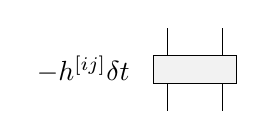
\begin{tikzpicture}
        \node[left] at (-5pt,5pt) {$\eto{-\im h^{[ij]} \delta t}$};
        \draw[draw, fill=gray!10] (0pt,0pt) rectangle (30pt,10pt);
        \draw (5pt,0pt) -- ++(0,-10pt);
        \draw (5pt,10pt) -- ++(0,10pt);
        \draw (25pt,0pt) -- ++(0,-10pt);
        \draw (25pt,10pt) -- ++(0,10pt);
    \end{tikzpicture}}}
    ~~ = ~~
    \vcenter{\hbox{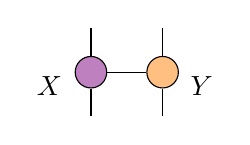
\begin{tikzpicture}[
            xt/.style={circle, draw, fill=violet!50, inner sep=0, minimum width=.4cm, minimum height=.4cm},
            yt/.style={circle, draw, fill=orange!50, inner sep=0, minimum width=.4cm, minimum height=.4cm},
        ]
        \node[xt] (X) at (0pt,0pt) {};
        \draw (X) -- ++(20pt,0) node[yt, right] (Y) {};
        \draw (X.south) -- ++(0,-10pt) (Y.south) -- ++(0,-10pt);
        \draw (X.north) -- ++(0,10pt) (Y.north) -- ++(0,10pt);
        \node at (-15pt,-5pt) {$X$};
        \node at (40pt,-5pt) {$Y$};
    \end{tikzpicture}}}
\end{equation}
of the bond gate in terms of two three-leg tensors.
%
Here, the superscript in brackets indicates which site is acted on, while the second superscript identifies the second site of the bond that $h^{[ij]}$ acts on.
%
Such a factorization is always possible at rank $\eta \leq d^2 = 4$ with (truncated) factorizations.
%
For the \acro{tfim} at finite filed strength $g > 0$, we require $\eta = 4$.
%
We can now define \acro{pepo} tensors
\begin{equation}
    \vcenter{\hbox{\begin{tikzpicture}
        \node[pepo tensor] (W3) {};
        \node[above left=3pt of W3] {$W^{[i]}$};
        \draw (C.north) -- ++(0, 5pt);
        \draw (C.south) -- ++(0, -5pt);
        \draw (C.west) -- ++(-10pt,0) node[left] {$l$};
        \draw (C.east) -- ++(10pt, 0) node[right] {$r$};
        \draw (C.north east) -- ++(5pt,5pt) node[above right] {$d$};
        \draw (C.south west) -- ++(-5pt,-5pt) node[below left] {$u$};
    \end{tikzpicture}}}
    ~~ := ~~
    \begin{cases}
        X^{[i],i+e_y}_u Y^{[i],i-e_y}_u X^{[i],i+e_x}_u Y^{[i],i-e_x}_u & i \in A \\
        Y^{[i],i-e_y}_u X^{[i],i+e_y}_u Y^{[i],i-e_x}_u X^{[i],i+e_x}_u & i \in B
    \end{cases}
    ~,
\end{equation}
where the difference between the cases for A and B sublattices is only a swapped order of the operators.
%
Note that we again suppress the physical indices associated with the vertical legs and associate them with the operators on the RHS.
%
As a result, a \acro{pepo}~\eqref{eq:tensornets:peps:pepo} built from these tensors realizes~\eqref{eq:gradpeps:tfim:evolution_op_bond_trotterization}.
%
To see this, consider the following patch of the larger \acro{pepo} network
\begin{equation}
    \vcenter{\hbox{\begin{tikzpicture}
        \node[pepo tensor] (W1) {};
        \draw (W1.east) -- ++(10pt,0) node[pepo tensor, right] (W2) {};
        \draw (W2.east) -- ++(10pt,0) node[pepo tensor, right] (W3) {};
        \draw (W3.east) -- ++(10pt,0) node[pepo tensor, right] (W4) {};
        \draw (W1.west) -- ++(-7pt,0);
        \draw (W4.east) -- ++(7pt,0);
        \draw (W1.north) -- ++(0,5pt);
        \draw (W2.north) -- ++(0,5pt);
        \draw (W3.north) -- ++(0,5pt);
        \draw (W4.north) -- ++(0,5pt);
        \draw (W1.south) -- ++(0,-5pt);
        \draw (W2.south) -- ++(0,-5pt);
        \draw (W3.south) -- ++(0,-5pt);
        \draw (W4.south) -- ++(0,-5pt);
        \draw (W1.north east) -- ++(5pt,5pt);
        \draw (W2.north east) -- ++(5pt,5pt);
        \draw (W3.north east) -- ++(5pt,5pt);
        \draw (W4.north east) -- ++(5pt,5pt);
        \draw (W1.south west) -- ++(-5pt,-5pt);
        \draw (W2.south west) -- ++(-5pt,-5pt);
        \draw (W3.south west) -- ++(-5pt,-5pt);
        \draw (W4.south west) -- ++(-5pt,-5pt);
    \end{tikzpicture}}}
    ~~ = ~~
    \vcenter{\hbox{\begin{tikzpicture}[
            xt/.style={circle, draw, fill=violet!50, inner sep=0, minimum width=.4cm, minimum height=.4cm},
            yt/.style={circle, draw, fill=orange!50, inner sep=0, minimum width=.4cm, minimum height=.4cm},
        ]
        \node[xt] (A1) {};
        \draw (A1.north) -- ++(0,10pt) node[yt, above] (A2) {};
        \draw (A2.north) -- ++(0,10pt) node[xt, above] (A3) {};
        \draw (A3.north) -- ++(0,10pt) node[yt, above] (A4) {};
        \draw (A4.north) -- ++(0,10pt) (A1.south) -- ++(0,-10pt);
        \node[yt, right=10pt of (A1)] (B1) {};
        \draw (B1.north) -- ++(0,10pt) node[xt, above] (B2) {};
        \draw (B2.north) -- ++(0,10pt) node[yt, above] (B3) {};
        \draw (B3.north) -- ++(0,10pt) node[xt, above] (B4) {};
        \draw (B4.north) -- ++(0,10pt) (B1.south) -- ++(0,-10pt);
        \node[xt, right=10pt of (B1)] (C1) {};
        \draw (C1.north) -- ++(0,10pt) node[yt, above] (C2) {};
        \draw (C2.north) -- ++(0,10pt) node[xt, above] (C3) {};
        \draw (C3.north) -- ++(0,10pt) node[yt, above] (C4) {};
        \draw (C4.north) -- ++(0,10pt) (C1.south) -- ++(0,-10pt);
        \node[yt, right=10pt of (C1)] (D1) {};
        \draw (D1.north) -- ++(0,10pt) node[xt, above] (D2) {};
        \draw (D2.north) -- ++(0,10pt) node[yt, above] (D3) {};
        \draw (D3.north) -- ++(0,10pt) node[xt, above] (D4) {};
        \draw (D4.north) -- ++(0,10pt) (D1.south) -- ++(0,-10pt);
        %
        \draw (A1.west) -- ++(-7pt, 0);
        \draw (A2.east) -- (B2.west) (B1.east) -- (C1.west) (C2.east) -- (D2.west);
        \draw (D1.east) -- ++(7pt, 0);
        \draw (A3.south west) -- ++(-5pt,-5pt);
        \draw (B4.south west) -- ++(-5pt,-5pt);
        \draw (C3.south west) -- ++(-5pt,-5pt);
        \draw (D4.south west) -- ++(-5pt,-5pt);
        \draw (A4.north east) -- ++(5pt,5pt);
        \draw (B3.north east) -- ++(5pt,5pt);
        \draw (C4.north east) -- ++(5pt,5pt);
        \draw (D3.north east) -- ++(5pt,5pt);
        %
        \begin{scope}[on background layer]
            \draw[draw=gray!80, fill=gray!10] ($(A2.north west)+(-3pt,3pt)$) rectangle ($(B2.south east)+(3pt,-3pt)$);
            \draw[draw=gray!80, fill=gray!10] ($(B1.north west)+(-3pt,3pt)$) rectangle ($(C1.south east)+(3pt,-3pt)$);
            \draw[draw=gray!80, fill=gray!10] ($(C2.north west)+(-3pt,3pt)$) rectangle ($(D2.south east)+(3pt,-3pt)$);
        \end{scope}
    \end{tikzpicture}}}
\end{equation}
and observe that the bond operators indicated by gray background boxes each multiply to the gate $\eto{-\im h^{[ij]} \delta t}$ on the respective bond.

As a result, we have constructed a \acro{pepo} for the evolution operator of the \acro{tfim} with bond dimension $\eta = 4$.


\paragraph{From product of MPOs}
Alternatively, we may first Trotterize between the group of horizontal and the group of vertical \acrop{mpo} in equation~\eqref{eq:gradpeps:benchmark:tfim_hamiltonian_as_mpos}.
%
Within these groups, the \acrop{mpo} mutually commute, and we can take the exponential of each \acro{mpo} according to the $W^{I/II}$ methods of Ref.~\cite{zaletel2014}.
%
The resulting \acro{mpo} has a bond dimension one smaller than for the corresponding Hamiltonian, i.e.~$\eta = 2$ for the \acro{tfim}.
% 
Assume that $C^{[x,y]}$ for $y=1,\dots, L$ are the \acro{mpo} tensors for the approximate exponential $\eto{-\im H^{[x,:]} \delta t}$ of the vertical \acro{mpo} on column $x$, and similarly $\tilde{C}^{[x,y]}$ the tensors for $\eto{-\im H^{[:,y]} \delta t}$ on row $y$.
%
We define a \acro{pepo} tensor as
\begin{equation}
    \vcenter{\hbox{\begin{tikzpicture}
        \node[pepo tensor] (W1) {};
        \draw (W1.west) -- ++(-7pt,0);
        \draw (W1.east) -- ++(7pt,0);
        \draw (W1.north) -- ++(0,5pt);
        \draw (W1.south) -- ++(0,-5pt);
        \draw (W1.north east) -- ++(5pt,5pt);
        \draw (W1.south west) -- ++(-5pt,-5pt);
        \node[above left=3pt of W1] {$W^{[x,y]}$};
    \end{tikzpicture}}}
    ~~ = ~~
    \vcenter{\hbox{\begin{tikzpicture}
        \node[pepo tensor, fill=lime!60] (W1) {};
        \draw (W1.north) -- ++(0,10pt) node[pepo tensor, fill=lime!60, above] (W2){};
        \draw (W2.west) -- ++(-7pt,0);
        \draw (W2.east) -- ++(7pt,0);
        \draw (W2.north) -- ++(0,5pt);
        \draw (W1.south) -- ++(0,-5pt);
        \draw (W1.north east) -- ++(5pt,5pt);
        \draw (W1.south west) -- ++(-5pt,-5pt);
        \node[below right=3pt of W1] {$C^{[x,y]}$};
        \node[above right=3pt of W2] {$\tilde{C}^{[x,y]}$};
    \end{tikzpicture}}}
    ~,
\end{equation}
which is designed such that on forming the \acro{pepo} tensor network, the \acro{mpo} tensors connect in such a way as to form the exponentials of row (column) Hamiltonians.
%
In particular, they parameterize a Trotterized time evolution \acro{pepo}
\begin{align}
\begin{split}
    \label{eq:gradpeps:tfim:evolution_pepo_from_WII}
    % \mathrm{PEPO}(\set{W^{[x,y]}})
    % &= \rBr{\prod_{y=1}^L \mathrm{MPO}(\tilde{C}^{[1,y]} \dots \tilde{C}^{[L,y]}) }
    % \!\rBr{\prod_{x=1}^L \mathrm{MPO}(C^{[x,1]} \dots C^{[x,L]}) }
    % \\
    % &\approx
    % \rBr{\prod_{y=1}^L \eto{-\im H^{[:,y]} \delta t}} \rBr{\prod_{x=1}^L \eto{-\im H^{[x,:]} \delta t}}
    % = \eto{-\im H_\text{hor} \delta t} \eto{-\im H_\text{vert} \delta t}
    % \\
    % &\approx\eto{-\im H \delta t}
    \eto{-\im H \delta t}
    &\approx 
    \eto{-\im H_\text{hor} \delta t} \eto{-\im H_\text{vert} \delta t}
    =
    \rBr{\prod_{y=1}^L \eto{-\im H^{[:,y]} \delta t}} \rBr{\prod_{x=1}^L \eto{-\im H^{[x,:]} \delta t}}
    \\
    &\approx
    \rBr{\prod_{y=1}^L \mathrm{MPO}(\tilde{C}^{[1,y]} \dots \tilde{C}^{[L,y]}) }
    \rBr{\prod_{x=1}^L \mathrm{MPO}(C^{[x,1]} \dots C^{[x,L]}) }
    \\[1ex]
    &= \mathrm{PEPO}(\set{W^{[x,y]}})
\end{split}
\end{align}
with bond dimension $\eta = 2$.
%
Again, the approximation is up to corrections in $\bigO(\delta t^2)$.


% ======================================================================
% ======================================================================
% ======================================================================
\subsection{Ground State Results}

As a benchmark of the gradient-based ground state search, we optimize ground state \acro{peps} for the \acro{tfim}~\eqref{eq:gradpeps:approx_contraction:results:ising_model} at a field strength $g=3$, which is close to criticality.
%
For an initial guess with bond dimension $D=2$, we apply a $D=2$ \acro{pepo}~\eqref{eq:gradpeps:tfim:evolution_pepo_from_WII} of a small step $\im\delta t = \delta\tau \sim 0.01$ of \emph{imaginary} time evolution to a $\sigma^z=+1$ product state.
%
We then optimize at this bond dimension by minimizing the variational energy~\eqref{eq:gradpeps:gradient_based:variational_energy} until convergence.
%
For optimizations at larger \acro{peps} bond dimension, we start from the $D=2$ result and increase its bond dimension, either by padding with zeroes or by applying another imaginary time step exactly.
%
In either case, we found it helpful for stability to introduce a small random perturbation and to apply a random gauge transformation on the bonds to avoid vanishing tensor entries.
%
Without this step, i.e.~just embedding a $D=2$ \acro{peps} into $D=3$, by padding with zeroes, all derivative components corresponding to these new slices will vanish, and we will be stuck at a saddle point for these entries.


\begin{table}[htp]
    \centering
    \begin{tabular}{llllll}
        \toprule
        $L$ & $D$ & This Work & FU & isoTNS & DMRG
        \\ \midrule
%%%%%%%%%%%%%%%%%%%%%%%%%%%%%%%%%%%%%%%%%%%%%%%%%%%%%%%%%%%%%%%%%%%%%%%%%%%	
        \multirow{3}{*}{11} & 2 &
        % L = 11 ; D = 2
            $-3.17185$ &  % This work
            $-3.17128$ &  % FU
            $-3.15546$ &  % isoTNS
            \multirow{3}{*}{$-3.17211$}  % DMRG
        \\
        & 3 &
        % L = 11 ; D = 3
            $-3.17185$ &  % This work
            $-3.17210$ &  % FU
             &  % isoTNS
        \\
        & 4 &
        % L = 11 ; D = 4
            $-3.17206$ &  % This work
            $-3.17210$ &  % FU
            $-3.16625$ &  % isoTNS
        \\ \midrule
        \multirow{3}{*}{20} & 2 &
        % L = 20 ; D = 2
            $-3.18138$ &  % This work
            &  % FU
            &  % isoTNS
            \multirow{3}{*}{$-3.18197$}  % DMRG
        \\
        & 3 &
        % L = 20 ; D = 3
            $-3.18138$ &  % This work
            &  % FU
            &  % isoTNS
        \\
        & 4 &
        % L = 20 ; D = 4
            $-3.18147$ &  % This work
            &  % FU
            &  % isoTNS
        \\ \midrule
%%%%%%%%%%%%%%%%%%%%%%%%%%%%%%%%%%%%%%%%%%%%%%%%%%%%%%%%%%%%%%%%%%%%%%%%%%%	
        \multirow{3}{*}{21} & 2 &
        % L = 21 ; D = 2
            $-3.18193$ &  % This work
            $-3.18128$ &  % FU
            &  % isoTNS
            \multirow{3}{*}{}  % DMRG
        \\
        & 3 &
        % L = 21 ; D = 3
            $-3.18193$ &  % This work
            $-3.18242$ &  % FU
            &  % isoTNS
        \\
        & 4 &
        % L = 21 ; D = 4
            $-3.18201$ &  % This work
            $-3.18243$ &  % FU
            &  % isoTNS
        \\ \bottomrule
    \end{tabular}
    \caption[
        Variational ground state energies of the TFIM.
    ]{
        \label{tab:gradpeps:gs}
        Variational ground state energy per site $E / L^2$ of the \acro{tfim} at $g=3$ on an $L \times L$
        square lattice with open boundary conditions.
        For this work and the Full Update (FU) algorithm\ \cite{lubasch2014a}, the variational manifold are PEPS with bond dimension $D$.
        The DMRG\textsuperscript{2} algorithm\ \cite{lin2022} (denoted isoTNS) finds a ground state approximation within
        the manifold of isometric PEPS of bond dimension $D$, a strict subset of all \acro{peps}.
        For comparison, we also give energies obtained from \acro{mps} calculation, using the \acro{dmrg} algorithm for which $D$ is meaningless.
        For the $11\times 11$ system, we used \acro{tenpy}~\cite{tenpySoftware, hauschild2024}, while the $20\times 20$ data was obtained in Ref.\ \cite{ganahl2023} using specialized hardware (\acrop{tpu}) and massive computational power at \acro{mps} bond dimension $2^{16} = 65536$.
    }
\end{table}




In table~\ref{tab:gradpeps:gs}, we compare variational energies as a measure of quality to other \acro{tns} methods.
%
At the lowest non-trivial bond dimension of $D=2$, we have achieved better ground state energies than any other \acro{peps} work we are aware of.
%
In particular, we improve upon the \acro{fu} results of Ref.~\cite{lubasch2014a} significantly and by more than the margin of error of the approximately evaluated energy.
%
We have fully converged the result at $L=11$, using a \acro{bmps} bond dimension $\chi_\text{max} = 300$ for the last few optimization steps close to the minimum, and evaluated the energies at $\chi_\text{max} = 350$.
%
We can conjecture with reasonable certainty that the result is, up to numerical precision, the global optimum within the manifold of \acro{peps} with bond dimension $D=2$.
%
For the larger systems, our proof-of-principle implementation reaches the limits of its computational performance.
%
Reaching a gradient norm of $\sim 0.1$ at $\chi_\text{max} = 200$, we are close to, but not fully converged, and still see change in the energy density on the fifth digit.
%
At the larger bond dimensions $D=3,4$, the results are not fully converged.
%
At $D=4$, we were only able to perform $\sim 100$ optimizer steps for $L=11$, and only $\sim 10$ steps for $L=20,21$ after applying an imaginary time step to the $D=2$ result.
%
We still obtain a competitive quality result.


% ======================================================================
% ======================================================================
% ======================================================================
\subsection{Time Evolution Results}


As a benchmark for the gradient-based time evolution algorithm, we simulate the time evolution induced by the \acro{tfim} Hamiltonian~\eqref{eq:gradpeps:approx_contraction:results:ising_model}
after a local quench.
%
For the quench, we apply $\sigma^y_{\vec{c}}$ to the central site $\vec{c}$ of a $11 \times 11$ lattice.
%
This constitutes a spin-flip excitation in both limits of the phase diagram.
%
We then simulate the dynamics
\begin{equation}
    \label{eq:gradpeps:approx_contraction:results:qunech_setup}
    \ket{\psi(t)}
    = \eto{-\im H t} \sigma^y_{\vec{c}} \GSket
\end{equation}
by applying a sequence of time steps $U(\delta t)$, giving us access to the evolved state at a grid of discrete times $t_n = n \delta t$.
%
We then extract the time-dependent correlation function
\begin{equation}
    \label{eq:gradpeps:approx_contraction:results:def_corr_func}
    C^{yy}(\vec{r}, t)
    := \braopket{\text{GS}}{\sigma^y_{\vec{r}}(t) \sigma^y_{\vec{c}}}{\text{GS}}
    .
\end{equation}



We evaluate it from the quench dynamics as
\begin{equation}
    \label{eq:gradpeps:approx_contraction:results:corr_func_evaluation}
    C^{yy}(\vec{r}, t_n + \tau)
    = \eto{\im E_0 \tau} \braopket{\text{GS}(t_n)}{\sigma^y_{\vec{r}} \eto{-\im H \tau}}{\psi(t_n)}
    .
\end{equation}
Here, we may explicitly include a time evolution operator for some smaller time step $\abs{\tau} \leq \delta t / 2$ to increase the resolution at which we evaluate the correlation function.
%
This is does not dominate the cost, as~\eqref{eq:gradpeps:approx_contraction:results:corr_func_evaluation} is a tensor network with the same structure as the cost function for time evolution.
%
It also allows for a consistency check of the approximate time evolution and Trotter approximation, where a kink in the data from $t_n + \tau_\text{max}$ to $t_{n+1} - \tau_\text{max}$ reveals problems in one of the two approximations.
%
Note that \acro{bmps} and partial contractions can be re-used between the evaluation for different positions $\vec{r}$.
%
We observe that it is beneficial to use the same time evolution method to explicitly evolve the ground state approximation instead of assuming that $\bra{\text{GS}} \eto{\im H t} = \eto{\im E_0 t} \bra{\text{GS}}$.
%
This is because (a) the ground state is only an approximation, and thus only approximately an energy eigenstate, and (b) the time evolution contains approximations and does not conserve energy exactly.
%



We then form the \acro{dsf}
\begin{equation}
    \label{eq:gradpeps:approx_contraction:results:def_dsf}
    S^{yy}(\vec{k},\omega) = \frac{1}{2\pi} \int_{-\infty}^{\infty} \d{t} ~ \sum_{\vec{r}} \eto{\im(\omega t - \vec{k}\cdot \vec{r})} C^{yy}(\vec{r}, t)
    .
\end{equation}
Let us first elaborate on the modifications needed to compute a proxy for the \acro{dsf} from the available data.
%
Firstly, to get access to correlation data for negative times, we may observe that in an infinite system with translational invariance, the correlation function fulfills
\begin{align}
    \begin{split}
        C^{yy}(\vec{r},-t)
        &= \braopket{\text{GS}}{\sigma^y_{\vec{r}}(0) \sigma^y_{\vec{c}}(t)}{\text{GS}}
        = \conj{\braopket{\text{GS}}{\sigma^y_{\vec{c}}(t) \sigma^y_{\vec{r}}(0)}{\text{GS}}}
        = \conj{C}^{yy}(-\vec{r},t)
        \\[1ex]
        &= \conj{C}^{yy}(\vec{r},t)
        ,
    \end{split}
\end{align}
where we used invariance of the ground state expectation value under time shifts, hermicity of the $\sigma^y$, translational invariance, and inversion symmetry.
%
As a result, we may evaluate the \acro{dsf} as
\begin{equation}
    \label{eq:gradpeps:tfim:dsf_with_int_over_only_positive times}
    S^{yy}(\vec{k},\omega) = \sum_{\vec{r}} \eto{-\im \vec{k}\cdot \vec{r}} \frac{1}{\pi} \int_{0}^{\infty} \d{t} ~ \mathrm{Re}\sBr{ \eto{\im\omega t} C^{yy}(\vec{r}, t)}
    ~.
\end{equation}
%
While this identity only holds for the infinite system, and translational invariance is not given for the finite system, we may choose to extrapolate the expression~\eqref{eq:gradpeps:tfim:dsf_with_int_over_only_positive times} to the thermodynamic limit instead of~\eqref{eq:gradpeps:approx_contraction:results:def_dsf}.
%
Alternatively, one could repeat the simulation to negative times by applying a sequence of $U(-\delta t)$ operators.


Secondly, we only have correlation data up to some finite cutoff time $T$, that is only for $t \leq T$.
%
Thus, for the time-to-frequency Fourier transform, e.g.~for a general function $f$ defined as
\begin{equation}
    \hat{f}(\omega) = \frac{1}{2\pi} \int_{-\infty}^\infty \d{t} ~ \eto{\im\omega t} f(t)
\end{equation}
we need to introduce some approximations to deal with the $\abs{t} > T$ integration range.
%
If we simply truncate the integration range, effectively including a windowing function $W(t) = \theta(T - \abs{t})$, we would find
\begin{equation}
    \frac{1}{2\pi} \int_{-T}^T \d{t} ~ \eto{\im\omega t} f(t)
    = \frac{1}{2\pi} \int_{-\infty}^\infty \d{t} ~ \eto{\im\omega t} f(t) W(t)
    = (\hat{f} * \hat{W})(\omega)
    ~,
\end{equation}
where $*$ denotes the convolution
\begin{equation}
    (\hat{f} * \hat{W})(\omega) = \int_{-\infty}^\infty \d{y} ~ \hat{f}(y) \hat{W}(\omega - y)
\end{equation}
of two functions.
%
We obtain the desired result $\hat{f}(\omega)$, but convoluted, i.e.~broadened by a sinc function $\hat{W}(\omega) = 2 / \omega \sin \omega T$.
%
This function has oscillating and slowly decaying tails around a main peak, such that sharp features in $\hat{f}(\omega)$ would be surrounded by ringing artifacts, which makes it difficult to interpret features.
%
We employ a common approach to avoid these by choosing a different windowing function, in particular, a Gaussian $W_\sigma(t) = \eto{-t^2/2\sigma^2}$ which results in convolution with
\begin{equation}
    \hat{W_\sigma}(\omega) = \sqrt{\frac{\sigma}{2 \pi}} \; \eto{-\sigma^2 \omega^2 / 2}
    ,
\end{equation}
i.e.~a Gaussian with width $1 / \sigma$.
%
This is a significant improvement since $\hat{W_\sigma}$ decays significantly faster, is strictly decreasing for $\omega > 0$, and is positive, such that convoluting with it does not introduce ringing and only smooths out the features.
%
We choose the width such that $W_\sigma(T) \ll 1$ is sufficiently decayed, such that we may truncate the integration range to $\abs{t} < T$ and introduce only a small error.


Lastly, we only have access to correlation data at discrete times, such that we need to discretize the integral.
%
Including these three modifications, we can evaluate the broadened structure factor as
\begin{equation}
    \hat{W_\sigma}(\omega) * S(\vec{k},\omega)
    \approx \sum_{\vec{r}} \eto{-\im\vec{k}\cdot\vec{x}} ~ \mathrm{Re}\sBr{\frac{1}{N}\sum_{n=0}^N \eto{\im\omega t_n} C^{yy}(\vec{r}, t_n)}
    .
\end{equation}
%
We present results for the \acro{dsf} from gradient-based time evolution in figure~\ref{fig:gradpeps:dsf}.
%
The extracted structure factor matches well with the perturbative dispersion relations.
%
At $g=3$, we see a small but significant gap of $\Delta \approx 1$ at the $\Gamma$ point.
%
We do not expect to see the gap close exactly because we simulate (i) slightly off criticality $g = 3 \lesssim g_c$, (ii) at finite system size, and (iii) at finite entanglement (due to the bounded bond dimension).
%
The results agree well with other works, such as isometric \acro{tns} in reference\ \cite{lin2022} and infinite \acro{peps} in reference~\cite{espinoza2024}, which perform very similar simulations of the \acro{dsf}, as well as qualitatively with the \acro{ipeps} excitation ansatz~\cite{vanderstraeten2019, ponsioen2020}, which extracts the excitation spectrum (i.e. the dispersion relation) in the thermodynamic limit.
%
We attribute the faint features above the main branch at $g=1,2$ to two-magnon bound states; the energy scale agrees with the result from the excitation ansatz\ \cite{ponsioen2020}.


\begin{figure}
    \centering
    \includegraphics[width=\linewidth]{graphics/gradpeps/dsf.pdf}
    \caption[
        Dynamical structure factor of the TFIM.
    ]{
        The dynamical structure factor $S^{yy}(\mathbf{k}, \omega)$ of the TFIM at different field strengths on an $11\times 11$ square lattice with open boundary conditions.
        %
	The horizontal axis describes a closed triangular path through the Brillouin zone with corners $\Gamma = (0,0)$, $X = (\tfrac{10}{11}\pi, 0)$, $M = (\tfrac{10}{11}\pi, \tfrac{10}{11}\pi)$.
        %
	The lines are the perturbative dispersions for low (blue) and high (green) field strengths, i.e.\ equations\ \eqref{eq:gradpeps:approx_contraction:results:perturbative_dispersion_low_g} and\ \eqref{eq:gradpeps:approx_contraction:results:perturbative_dispersion_high_g}.
	%
	The width $\sigma_\omega$ of the Gaussian broadening that we artificially introduce is indicated in the left panel.
    }
    \label{fig:gradpeps:dsf}
\end{figure}


We can obtain a reference for the \acro{dsf} from perturbative calculations.
%
In the limit of small transverse fields, $g \ll g_c$, the elementary excitations on top of the $\sigma^x$ polarized ground state are single spin flips, and the simulated quench does indeed create such an excitation.
%
Now, second-order time-dependent perturbation theory in the field term results in a hopping model of these spin flips, where nearest neighbor hopping is favored since the intermediate virtual state of two neighboring spin flips dissatisfies the interaction term on only six bonds, compared to the eight bonds for other configurations.
%
In the opposite limit $g \gg g_c$, the quench also induces a spin-flip, this time on top of a $\sigma^x = +1$ polarized ground state, and we directly find a nearest neighbor hopping model of the spin flips in first-order perturbation theory of the interaction term.
%
In both cases, we find sharp features
\begin{equation}
    \label{eq:gradpeps:approx_contraction:results:expected_dsf}
    S^{yy}(\vec{k},\omega) = \delta( \omega - \epsilon(\vec{k}) )
\end{equation}
in the structure factor with weight on the dispersion relations, which are given by
\begin{align}
    \label{eq:gradpeps:approx_contraction:results:perturbative_dispersion_low_g}
    \epsilon_{g \ll g_c}(\mathbf{k}) 
    &= 8 - \frac{g^2}{4}\left[1 + \cos k_x + \cos k_y\right]+ \bigO\left(g^3\right)
    \\
    \label{eq:gradpeps:approx_contraction:results:perturbative_dispersion_high_g}
    \epsilon_{g \gg g_c}(\mathbf{k}) 
    &= 2g \left(1 - \frac{1}{g}\left[\cos k_x + \cos k_y\right] + \bigO\left(\frac{1}{g^2}\right)\right)
    .
\end{align}
These dispersion relations are overlayed in figure~\ref{fig:gradpeps:dsf} for comparison.
